\chapter{Review of Related Work}

\label{chapter:mapping}

In Chapter \ref{section:cnn_flattening}, we discussed how convolutional neural networks (CNNs) can be flattened into matrix-matrix multiplications. Most ML software and accelerators use this matrix-matrix multiplication using the im2col transformation to implement convolutions.

\begin{figure}[htbp]
    \centering
    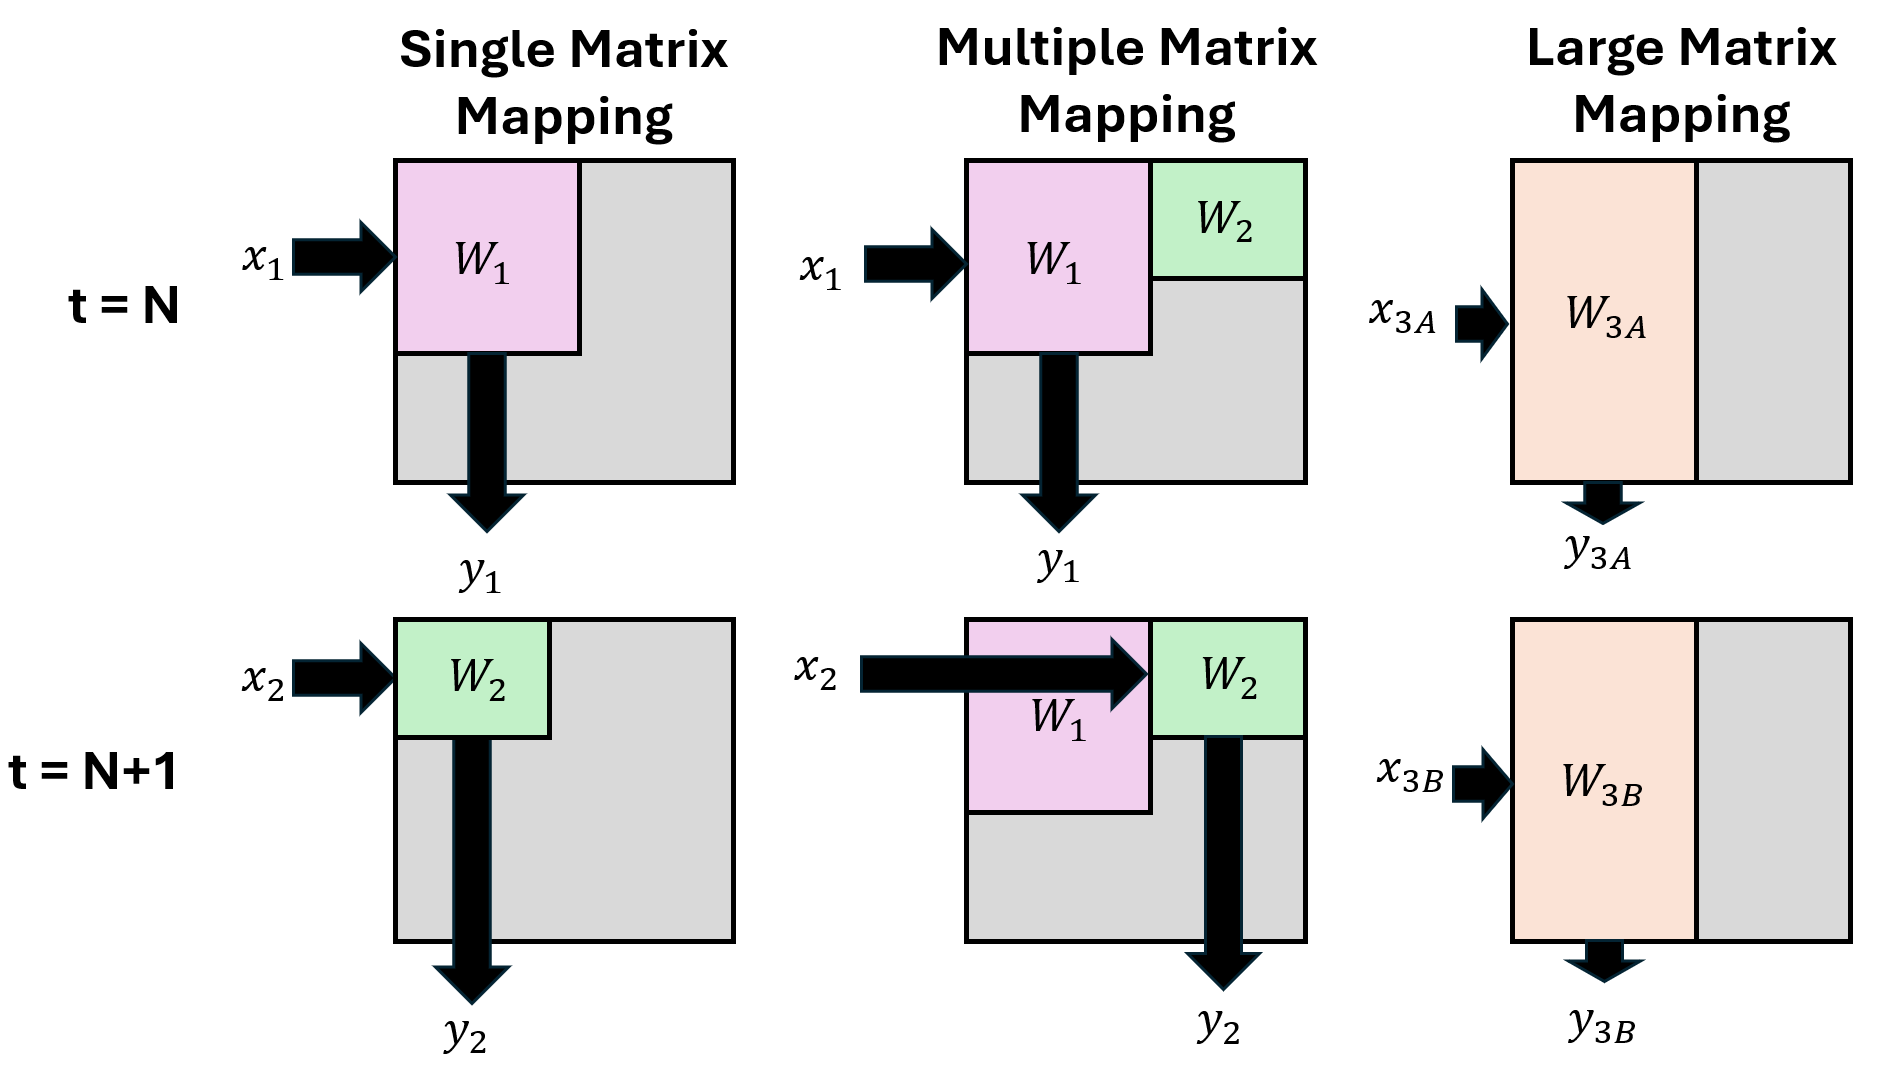
\includegraphics[width=0.8\textwidth]{images/mapping/mapping_single.png}
    \caption{Matrix mapping onto AIMC}
    \label{fig:mapping_single}
\end{figure}

When an AIMC accelerator performs an MVM operation, the matrix must first be mapped into the AIMC memory array, as in Figure \ref{fig:mapping_single} (left). In the rest of this thesis, we will be calling the mapped matrices "bins". The weights $W_1$ are written into the AIMC memory array. Then, the input vector $x_1$ is applied row-rise to the AIMC memory array (also as analog signals) in a way that is aligned with the mapped matrix $W_1$. After this, the analog result signals $y_1$ are read out from the AIMC memory array completing the matrix-vector multiplication.

The AIMC can also map multiple matrices at the same time, as in Figure \ref{fig:mapping_single} (middle). This way, the AIMC can time-multiplex the use of either weight matrix $W_1$ or $W_2$. This results in effectively the same amount of time to perform the MVM operation as if the AIMC only mapped a single matrix. However, this approach requires writing into the memory array only once as opposed to twice in the single-matrix example.

When the matrix to be mapped is larger than the AIMC memory array, the matrix can be split into two matrices $W_3 = \begin{bmatrix} W_{3A} \\ W_{3B} \end{bmatrix}$. Then, the output each section of the operation can be added together as $y_3=y_{3a} + y_{3b}$ to get the final output, as in Figure \ref{fig:mapping_single} (right). For cases where the matrix is horizontally split, $y_3 = \begin{bmatrix} y_{3a} y_{3b} \end{bmatrix}$. Hence, AIMCs can map any matrix size into their array given enough time to perform the MVM operation.


\begin{figure}[htbp]
    \centering
    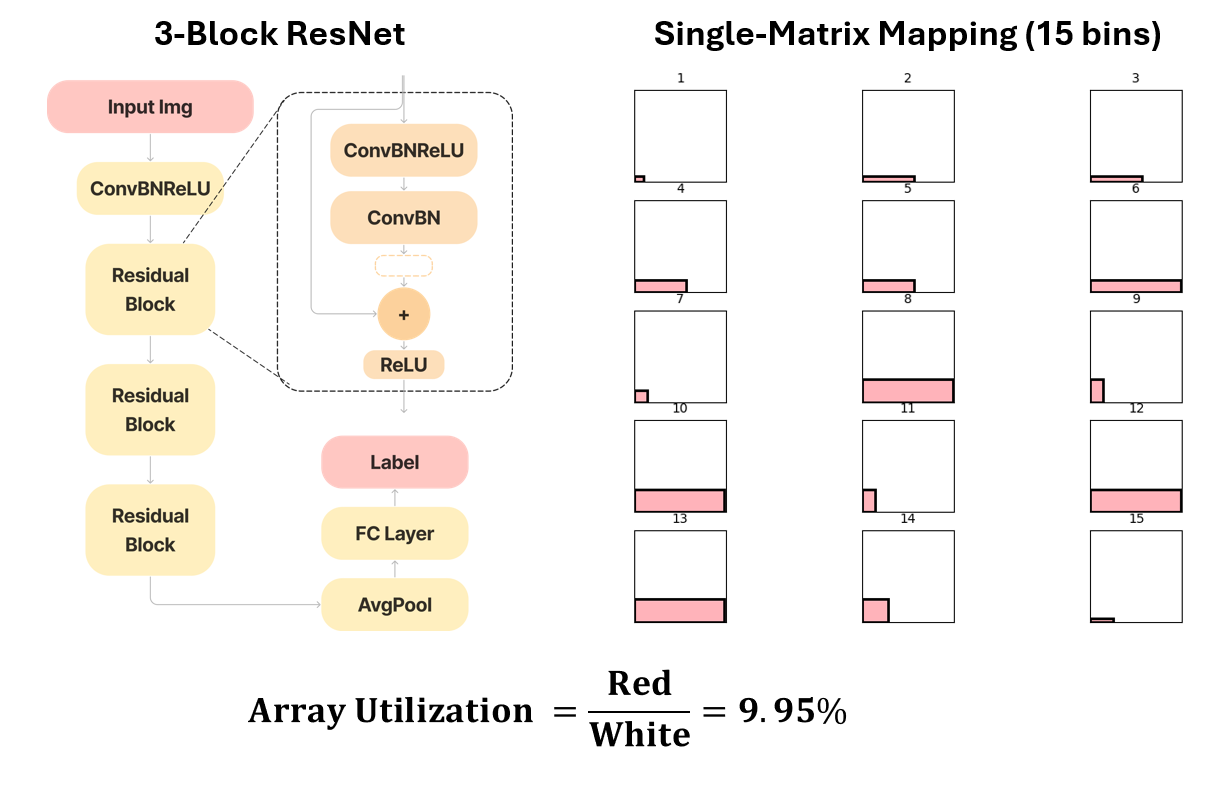
\includegraphics[width=0.8\textwidth]{images/mapping/resnet_singlemapping.png}
    \caption{Single-mapping of a 3-block ResNet-18 into AIMC. The AIMC array utilization is at 9\% with single-mapping.}
    \label{fig:resnet_singlemapping}
\end{figure}

\section{AIMC Utilization}

In the single-mapping scheme, the mapped matrix utilizes $\frac{CK}{N_{rows}N_{cols}}$ of the AIMC memory array if the matrix $W_1$ is of size $K \times C$ and the AIMC memory array is of size $N_{rows} \times N_{cols}$. Figure \ref{fig:resnet_singlemapping} shows an example of a single-mapping of MLPerfTiny's 3-block ResNet-18 into an AIMC array. Because of the diversity of matrix sizes composing the DNN models, the AIMC utilization is typically very low for most parameter-efficient DNNs. Table \ref{table:single_mapping_utilization} shows the AIMC utilization of the MLPerfTiny models on a $256x256$ AIMC core when mapped using single-mapping. When larger cores are utilized, the utilization gets even lower (more free space). On the other hand, smaller AIMC cores result in a higher utilization, but they would also be less energy-efficient as small AIMC cores are less able to amortize the costs of their peripheral circuitry \cite{murmann2020mixed}.

\begin{table}[h]
\caption{Single-mapping utilization of the MLPerfTiny models on AIMC}
\label{table:single_mapping_utilization}
\centering
\begin{tabular}{ccc}
\cline{2-3}
\multicolumn{1}{c|}{} & \multicolumn{2}{c}{\textbf{Core Size}}    \\ \hline
\textbf{Model}        & \textbf{(256, 256)} & \textbf{(512, 512)} \\ \hline
DS-CNN                & 5.01\%              & 1.25\%              \\
MobileNetV2           & 35.86\%             & 15.69\%             \\
ResNet                & 9.95\%              & 3.39\%              \\
FC-AutoEncoder        & 28.79\%             & 8.40\%             
\end{tabular}%
\end{table}

More important is the number of AIMC memory writes required to perform an entire inference. Each bin in Figure \ref{fig:resnet_singlemapping} is a full write onto the AIMC for which only the red portion is the useful portion of the matrix. Hence, for a single core AIMC, 15 full writes onto the AIMC are needed for a full ResNet inference. For multicore AIMC, it can be interpreted as needing 15 cores to map the entire ResNet-18 model (or, in cases where there are less than 15 cores, needing to evict some of the written mappings to write new ones).

This is a significant problem for AIMC accelerators if you consider the fact that common AIMC memory types such as SRAM, FEFET, and MTJ can have write energies that are much greater than the energy used to perform computations with them. Table \ref{table:aimc_memory_write_energy} shows the write energy and time of the most popular memory types used for AIMC.

\begin{table}[h]
\caption{AIMC memory write energy and time (Data from 2024 \cite{meng2024compute})}
\label{table:aimc_memory_write_energy}
\centering
% \resizebox{\columnwidth}{!}{%
\begin{tabular}{lll}
\hline
\textbf{Memory Type} & \textbf{Write Energy} & \textbf{Write Time} \\ \hline
SRAM                 & $\sim$1 fJ            & $\sim$1 ns          \\
FEFET                & $\sim$1 fJ            & 100 ns              \\
MTJ                  & $\sim$100 fJ          & $\sim$10 ns         \\
PCM                  & $\sim$10 000 fJ       & $\sim$50 ns         \\
RRAM                 & $\sim$1 000 fJ        & $\sim$100 ns       
\end{tabular}%
% }
\end{table}

For that reason, multi-mapping schemes are more desirable for AIMC. By mapping multiple matrices into one mapped matrix decreasing the number of mapped matrices and the number of mapped matrix writes onto the AIMC is desirable. As will be discussed in the next section, multi-mapping schemes are not commonly used in mappers for DNN workloads.

\section{Mappers of DNN Workloads}

Numerous previous works exist on automatically mapping DNN models to accelerators. Table \ref{table:mappers} summarizes these works. However, most system-level mapping optimizers that can account for AIMC (ZigZag \cite{mei2021zigzag}, Stream \cite{symons2024stream}, CIMLoop \cite{andrulis2024cimloop}, NeuroSIM \cite{chen2018neurosim}) limit themselves to single-mapping schemes. Most of these works use single-mapping to simplify the treatment of AIMC accelerators, in a way treating them like digital accelerators. 

\begin{table}[h]
\label{table:mappers}
\caption{Comparison of DNN mapping optimizers}
\resizebox{\columnwidth}{!}{%
\begin{tabular}{ccccccc}
\hline
\textbf{} &
  \textbf{NeuroSIM (2019)} &
  \textbf{\begin{tabular}[c]{@{}c@{}}Kourtis et al.\\(2020)\end{tabular}} &
  \textbf{\begin{tabular}[c]{@{}c@{}}CIMLoop\\(2024)\end{tabular}} &
  \textbf{\begin{tabular}[c]{@{}c@{}}Stream/ZigZag\\(2024)\end{tabular}} &
  \textbf{\begin{tabular}[c]{@{}c@{}}LionHeart\\(2025)\end{tabular}} &
  \textbf{\begin{tabular}[c]{@{}c@{}}MARP\\(This Work)\end{tabular}} \\ \hline 
\begin{tabular}[c]{@{}c@{}}Mapping\\Type\end{tabular}         & Single & Single & Single & Single & Single & \cellcolor[HTML]{9AFF99}Multiple \\
\begin{tabular}[c]{@{}c@{}}Target\\Hardware\end{tabular}      & AIMC   & AIMC   & AIMC   & Hybrid & Hybrid & \cellcolor[HTML]{9AFF99}Hybrid   \\
\begin{tabular}[c]{@{}c@{}}Caching\\Optimization?\end{tabular} & No     & No     & Yes    & Yes    & No     & \cellcolor[HTML]{FFCCC9}No       \\
\begin{tabular}[c]{@{}c@{}}Latency\&\\Energy Modelling?\end{tabular}       & Yes    & No     & Yes    & Yes    & Yes    & \cellcolor[HTML]{9AFF99}Yes     
\end{tabular}%
}
\end{table}

\subsubsection{Optimized Mappers are limited to Single-Mapping Schemes}

NeuroSIM \cite{chen2018neurosim} is an AIMC accelerator simulator that simulates the performance of AIMC accelerators with a specific architecture hierarchy. Because of that, it has flexible models to predict the energy and latency of AIMC accelerators while also potentially allowing the user to specify the mapped workloads. However, they limit themselves to mapping a single layer per AIMC core to simplify the workload mapping and data routing problems.

ZigZag \cite{mei2021zigzag} optimizes the mapping of weights, input features, and output features on various DNN accelerator dataflows including AIMCs. Various accelerators can use ZigZag to optimize the allocation of weights and feature maps to the accelerator memory hierarchy. At the same time, ZigZag's latency and energy models allow it to create optimal architectures for AIMC accelerators. For example, the earlier mentioned DIANA \cite{houshmand2022diana} was optimized using ZigZag. However, in its models and predictions, ZigZag can only optimize a single layer at a time due to significant complexity introduced when accounting for interlayer data reuse. 

Stream \cite{symons2024stream} builds on ZigZag's work by accounting for interlayer data reuse in AIMC accelerators. Stream can account for data dependencies between layers to optimize the mapping and order of workloads in the AIMC accelerator. However, as it is built on ZigZag, it also only supports single-mapping schemes.

MIT's CIMLoop \cite{andrulis2024cimloop} is a DNN mapper for AIMC accelerators that is based on MIT's TimeLoop \cite{parashar2019timeloop}. Like ZigZag, TimeLoop only optimized dataflow and workload mapping single layers. Hence, CIMLoop could only also account for and optimize the energy and latency of single layers.

LionHeart \cite{lammie2024lionheart} chooses to optimize model performance in the mapping of DNNs to hybrid accelerators by selectively choosing to map layers with low precision requirements to AIMC accelerators and layers with high precision requirements to digital accelerators. However, as a way to simplify the problem complexity, LionHeart also only supports single-mapping schemes. 

\subsubsection{Some AIMC works use multi-mapping schemes but only for demonstration}

However, this is not to say that multi-mapping has never been explored. Multi-mapping schemes are sometimes used to demonstrate the feasibility of inference with AIMC accelerator works. For example, NeuRRAM \cite{wanneurram} utilizes an ad-hoc heuristic mapping scheme for the models that they used to demonstrate their work. The downside is that their mapping is handcrafted to produce low inference latency for their accelerator. NeuRRAM gives utilization a lower priority, and achieves utilizations of only about 4\%-38.3\%. This is partly because they have 48 cores which is more than enough to map the entire models without eviction. Unfortunately, most other AIMC accelerators usually only have a single core and it may be generally infeasible to integrate such a large number of AIMC cores alongside other functionalities inside a system-on-chip (SoC) on an edge device.

Garofalo et al. \cite{garofalo2022heterogeneous} also used multi-mapping to demonstrate the feasibility of mapping the entire MobileNetV2 model into their heterogenous accelerator. Moreover, they use rectangular packing to obtain an optimally dense mapping. However, they only used it to demonstrate the feasibility of mapping MobileNetV2 onto their accelerator. They provided no analysis of mapping optimization, energy effiency gains, and latency. Not only that, but they only demonstrate the final mapping of a single model.

Furthermore, these mapping schemes are only used once to demonstrate the feasibility of the AIMC accelerator. There exists a need for true multi-mapping DNN mapper that supports many DNN models. There is also a significant need to find optimal multi-mapping schemes in terms of energy efficiency, latency, and array utilization.